\documentclass{beamer}

\usetheme{Madrid}
\usecolortheme{default}

\usepackage{amsmath}
\usepackage{amssymb}
\usepackage{graphicx}
\usepackage{listings}

\title{Graduate Algorithms}
\subtitle{Tutorial 1: Math for Algorithms}
\author{}
\date{\today}

\begin{document}

\frame{\titlepage}

% ============================================================================
% INTRODUCTION SECTION
% ============================================================================

\section{Introduction}

\begin{frame}
  \frametitle{Why Study Algorithms?}
  Two undeniably true things about the human experience:
  \begin{enumerate}
    \item We are absolutely surrounded by problems
    \item Our time is far too limited to spend forever solving them
  \end{enumerate}
  
  \vspace{0.5cm}
  
  \textbf{This is the entire motivation for the study of algorithms.}
  
  \vspace{0.3cm}
  
  Long before computers existed, people developed algorithms for arithmetic, navigation, voting, logistics, and trade.
  
  Computers simply gave us the ability to apply those ideas at impossible scales.
\end{frame}

\begin{frame}
  \frametitle{Key Questions in Algorithms}
  
  In this course, we'll study how to think about problems efficiently.
  
  \begin{itemize}
    \item How do we compare different solutions?
    \item What makes one algorithm faster than another?
    \item How do we model complicated real-world situations?
    \item When is a problem easy, and when is it fundamentally difficult?
    \item How do we deal with 'difficult' problems?
  \end{itemize}
  
  \vspace{0.3cm}
  
  \textit{The world is full of problems. Might as well get good at solving them.}
\end{frame}

% ============================================================================
% ASYMPTOTICS SECTION
% ============================================================================

\section{Asymptotics}

\begin{frame}
  \frametitle{Asymptotic Dominance}
  
  \begin{definition}
    Asymptotic Dominance is a relation over functions, where $f(n) \prec g(n)$ when $g(n)$ approaches infinity faster than $f(n)$:
    
    $$f(n) \prec g(n) \iff \limsup_{n \to \infty} \frac{|f(n)|}{|g(n)|} = 0$$
    
    Furthermore, $f(n) \asymp g(n) \iff \limsup_{n \to \infty} \frac{|f(n)|}{|g(n)|} = k$ where $0 < k < \infty$ is constant.
  \end{definition}
\end{frame}

\begin{frame}
  \frametitle{Properties of Asymptotic Dominance}
  
  \begin{corollary}
    Asymptotic dominance is transitive.
  \end{corollary}
  
  \begin{corollary}
    If $\alpha < \beta$ then $x^\alpha \prec x^\beta$
  \end{corollary}
  
  \begin{corollary}
    Let $f(x) = k \cdot g(x)$ for some real $k \neq 0$, then $f(x) \asymp g(x)$
  \end{corollary}
  
  \vspace{0.3cm}
  
  \textbf{Key insight:} In a sum of functions, we only need to consider the most dominant function. We can talk about groups of functions using a single 'representative' function.
\end{frame}

\begin{frame}
  \frametitle{Representative Function}
  
  \begin{definition}
    The representative function of a set of asymptotically equivalent functions is:
    \begin{itemize}
      \item A function with a leading coefficient of $1$
      \item No additive subdominant terms
    \end{itemize}
    
    For example: $x^2$ is the representative function of the equivalence class of quadratic functions $ax^2 + bx + c$.
  \end{definition}
\end{frame}

\begin{frame}
  \frametitle{Theorem: Representative Functions}
  
  \begin{theorem}
    If $f(x), g(x)$ are representative functions of equivalence classes $F, G$; then 
    $$f(x) \succ g(x) \iff \hat{f}(x) \succ \hat{g}(x)$$ 
    for all $\hat{f} \in F$ and $\hat{g} \in G$
  \end{theorem}
  
  \vspace{0.3cm}
  
  This means the asymptotic ordering is \textbf{invariant under scaling and translation by dominated functions}.
\end{frame}

\begin{frame}
  \frametitle{Exercise: Hierarchy of Common Functions}
  
  Prove that:
  $$1 \prec \log \log n \prec \log n \prec n^\epsilon \prec n^c \prec n^{\log n} \prec c^n \prec n! \prec n^n \prec c^{c^n}$$
  
  where $\epsilon, c$ are small positive constants.
\end{frame}

\begin{frame}
  \frametitle{Big Oh Notation (Definition 1)}
  
  \begin{definition}[Big Oh (from hierarchy)]
    $$f(n) = O(g(n)) \iff f(n) \preceq g(n)$$
  \end{definition}
  
  \begin{definition}[Big Oh (limit)]
    $$f(n) = O(g(n)) \iff \limsup_{n \to \infty} \frac{|f(n)|}{|g(n)|} < \infty$$
  \end{definition}
  
  \begin{definition}[Big Oh (Classical)]
    $$f(n) = O(g(n)) \iff \exists c, n_0 \text{ s.t. } \forall n \geq n_0, |f(n)| \leq c \cdot |g(n)|$$
  \end{definition}
\end{frame}

\begin{frame}
  \frametitle{Bachmann-Landau Notation}
  
  \begin{center}
    \begin{tabular}{|l|l|}
      \hline
      \textbf{Notation} & \textbf{Name} \\
      \hline
      $f(n) = \Theta(g(n))$ & Big Theta \\
      $f(n) = \Omega(g(n))$ & Big Omega \\
      $f(n) \sim g(n)$ & Total Asymptotic Equivalence \\
      $f(n) = o(g(n))$ & Small Oh \\
      $f(n) = \omega(g(n))$ & Small Omega \\
      \hline
    \end{tabular}
  \end{center}
\end{frame}

\begin{frame}
  \frametitle{Example: $3n^2 - 100n + 6$}
  
  \begin{itemize}
    \item $3n^2 - 100n + 6 = O(n^2)$ ✓
    \item $3n^2 - 100n + 6 = O(n^3)$ ✓
    \item $3n^2 - 100n + 6 \neq O(n)$ ✗
    \item $3n^2 - 100n + 6 = \Omega(n^2)$ ✓
    \item $3n^2 - 100n + 6 \neq \Omega(n^3)$ ✗
    \item $3n^2 - 100n + 6 = \Theta(n^2)$ ✓
    \item $3n^2 - 100n + 6 \neq \Theta(n^3)$ ✗
  \end{itemize}
  
  \vspace{0.3cm}
  
  Also: $3n^2 - 100n + 6 \sim 3n^2$ by taking the limit.
\end{frame}

\begin{frame}
  \frametitle{Exercise: Big Oh Arithmetic}
  
  Prove the following:
  \begin{enumerate}
    \item $n^m = O(n^{m'})$ for $m \leq m'$
    \item $O(f(n)) + O(g(n)) = O(|f(n)| + |g(n)|)$
    \item $f(n) = O(f(n))$
    \item $O(O(f(n))) = O(f(n))$
    \item $c \cdot O(f(n)) = O(f(n))$ for constant $c$
    \item $O(f(n)) \cdot O(g(n)) = O(f(n)g(n))$
    \item $O(f(n)^2) = O(f(n))^2$
  \end{enumerate}
\end{frame}

\begin{frame}
  \frametitle{Sum of Powers: Asymptotic Behavior}
  
  \begin{exampleblock}{Example}
    Consider $f_k(n) = \sum_{i=1}^n i^k$ for $k, n \in \mathbb{N}$.
    
    Small cases:
    \begin{align*}
      f_0(n) &= \sum_{i=1}^n 1 = n = O(n) \\
      f_1(n) &= \sum_{i=1}^n i = \frac{n(n+1)}{2} = O(n^2) \\
      f_2(n) &= \sum_{i=1}^n i^2 = \frac{n(n+1)(2n+1)}{6} = O(n^3)
    \end{align*}
  \end{exampleblock}
\end{frame}

\begin{frame}
  \frametitle{Theorem: Sum of Powers}
  
  \begin{theorem}
    For all $k \geq 0$:
    $$f_k(n) = \sum_{i=1}^n i^k = O(n^{k+1})$$
  \end{theorem}
  
\end{frame}

\begin{frame}
  \frametitle{Proof: Sum of Powers}
  
    \begin{proof}
    \begin{align*}
      f_k(n) &= \sum_{i=1}^n i^k \\
      &= \sum_{i=1}^n O(n^k) \\
      &= n \cdot O(n^k) \\
      &= O(n^{k+1})
    \end{align*}
  \end{proof}

   This proof is simpler than induction!
  
\end{frame}

% ============================================================================
% GRAPH THEORY SECTION
% ============================================================================

\section{Graph Theory}

\begin{frame}
  \frametitle{Why Graphs?}
  
  Statements we often hear:
  \begin{itemize}
    \item ``Your friends, on average, have more friends than you''
    \item ``Any 2 people can be connected to each other in 6 relations''
  \end{itemize}
  
  \vspace{0.3cm}
  
  One way to reason about networks (people, roadways, etc.) is through \textbf{Graphs}.
  
  \vspace{0.3cm}
  
  We'll formalize and prove such claims using graph theory.
\end{frame}

\begin{frame}
  \frametitle{Simple Graph}
  
  \begin{definition}
    A (simple) graph is an ordered pair $G = (V, E)$ where:
    \begin{itemize}
      \item $V$ is the set of \textbf{vertices}
      \item $E \subseteq \{\{x, y\} \mid x, y \in V, x \neq y\}$ is a set of unordered pairs called \textbf{edges}
    \end{itemize}
  \end{definition}
  
  Visualization: Each vertex is a point in the plane; each edge is a line between corresponding vertices.
\end{frame}

\begin{frame}
  \frametitle{Directed Graph}
  
  \begin{definition}
    In a directed graph, $E \subseteq \{(x, y) \mid x, y \in V, x \neq y\}$. The pairs are ordered, making the edges \textbf{directed}.
  \end{definition}
  
  Visualization: Edges are drawn with arrowheads to indicate direction.
\end{frame}

\begin{frame}
  \frametitle{Weighted (Directed) Graph}
  
  \begin{definition}
    A (directed) graph with a function $w : E \to \mathbb{R}$ is called a weighted (directed) graph.
  \end{definition}
  
  This allows modeling real-world quantities like distances, costs, or capacities.
\end{frame}

\begin{frame}
  \frametitle{Example: Karate Club Network}
  
  \begin{center}
    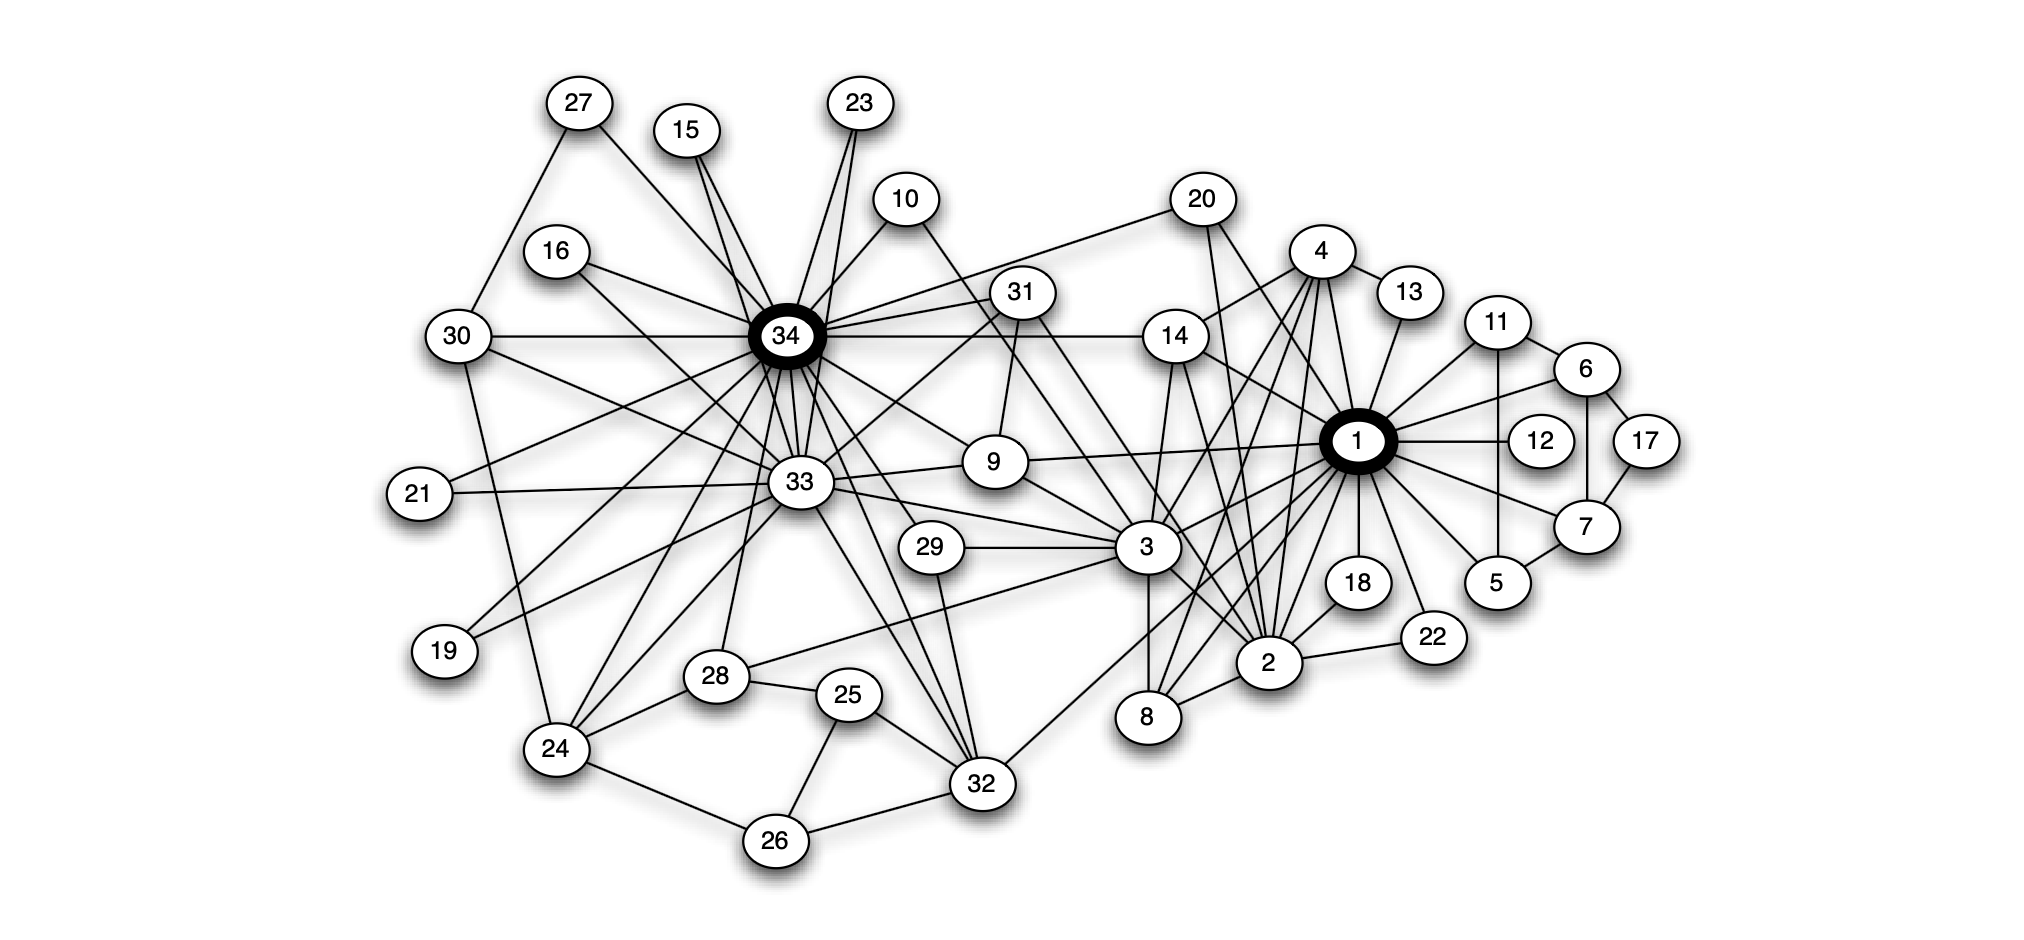
\includegraphics[width=0.6\textwidth]{karate-club.png}
  \end{center}
  
  The social network of friendships within a 34-person karate club.
  
  \textit{Questions:} If we wanted to spread a rumor quickly, where would we start? How to split the club?
\end{frame}

\begin{frame}
  \frametitle{Example: Delhi Metro}
  
  \begin{center}
    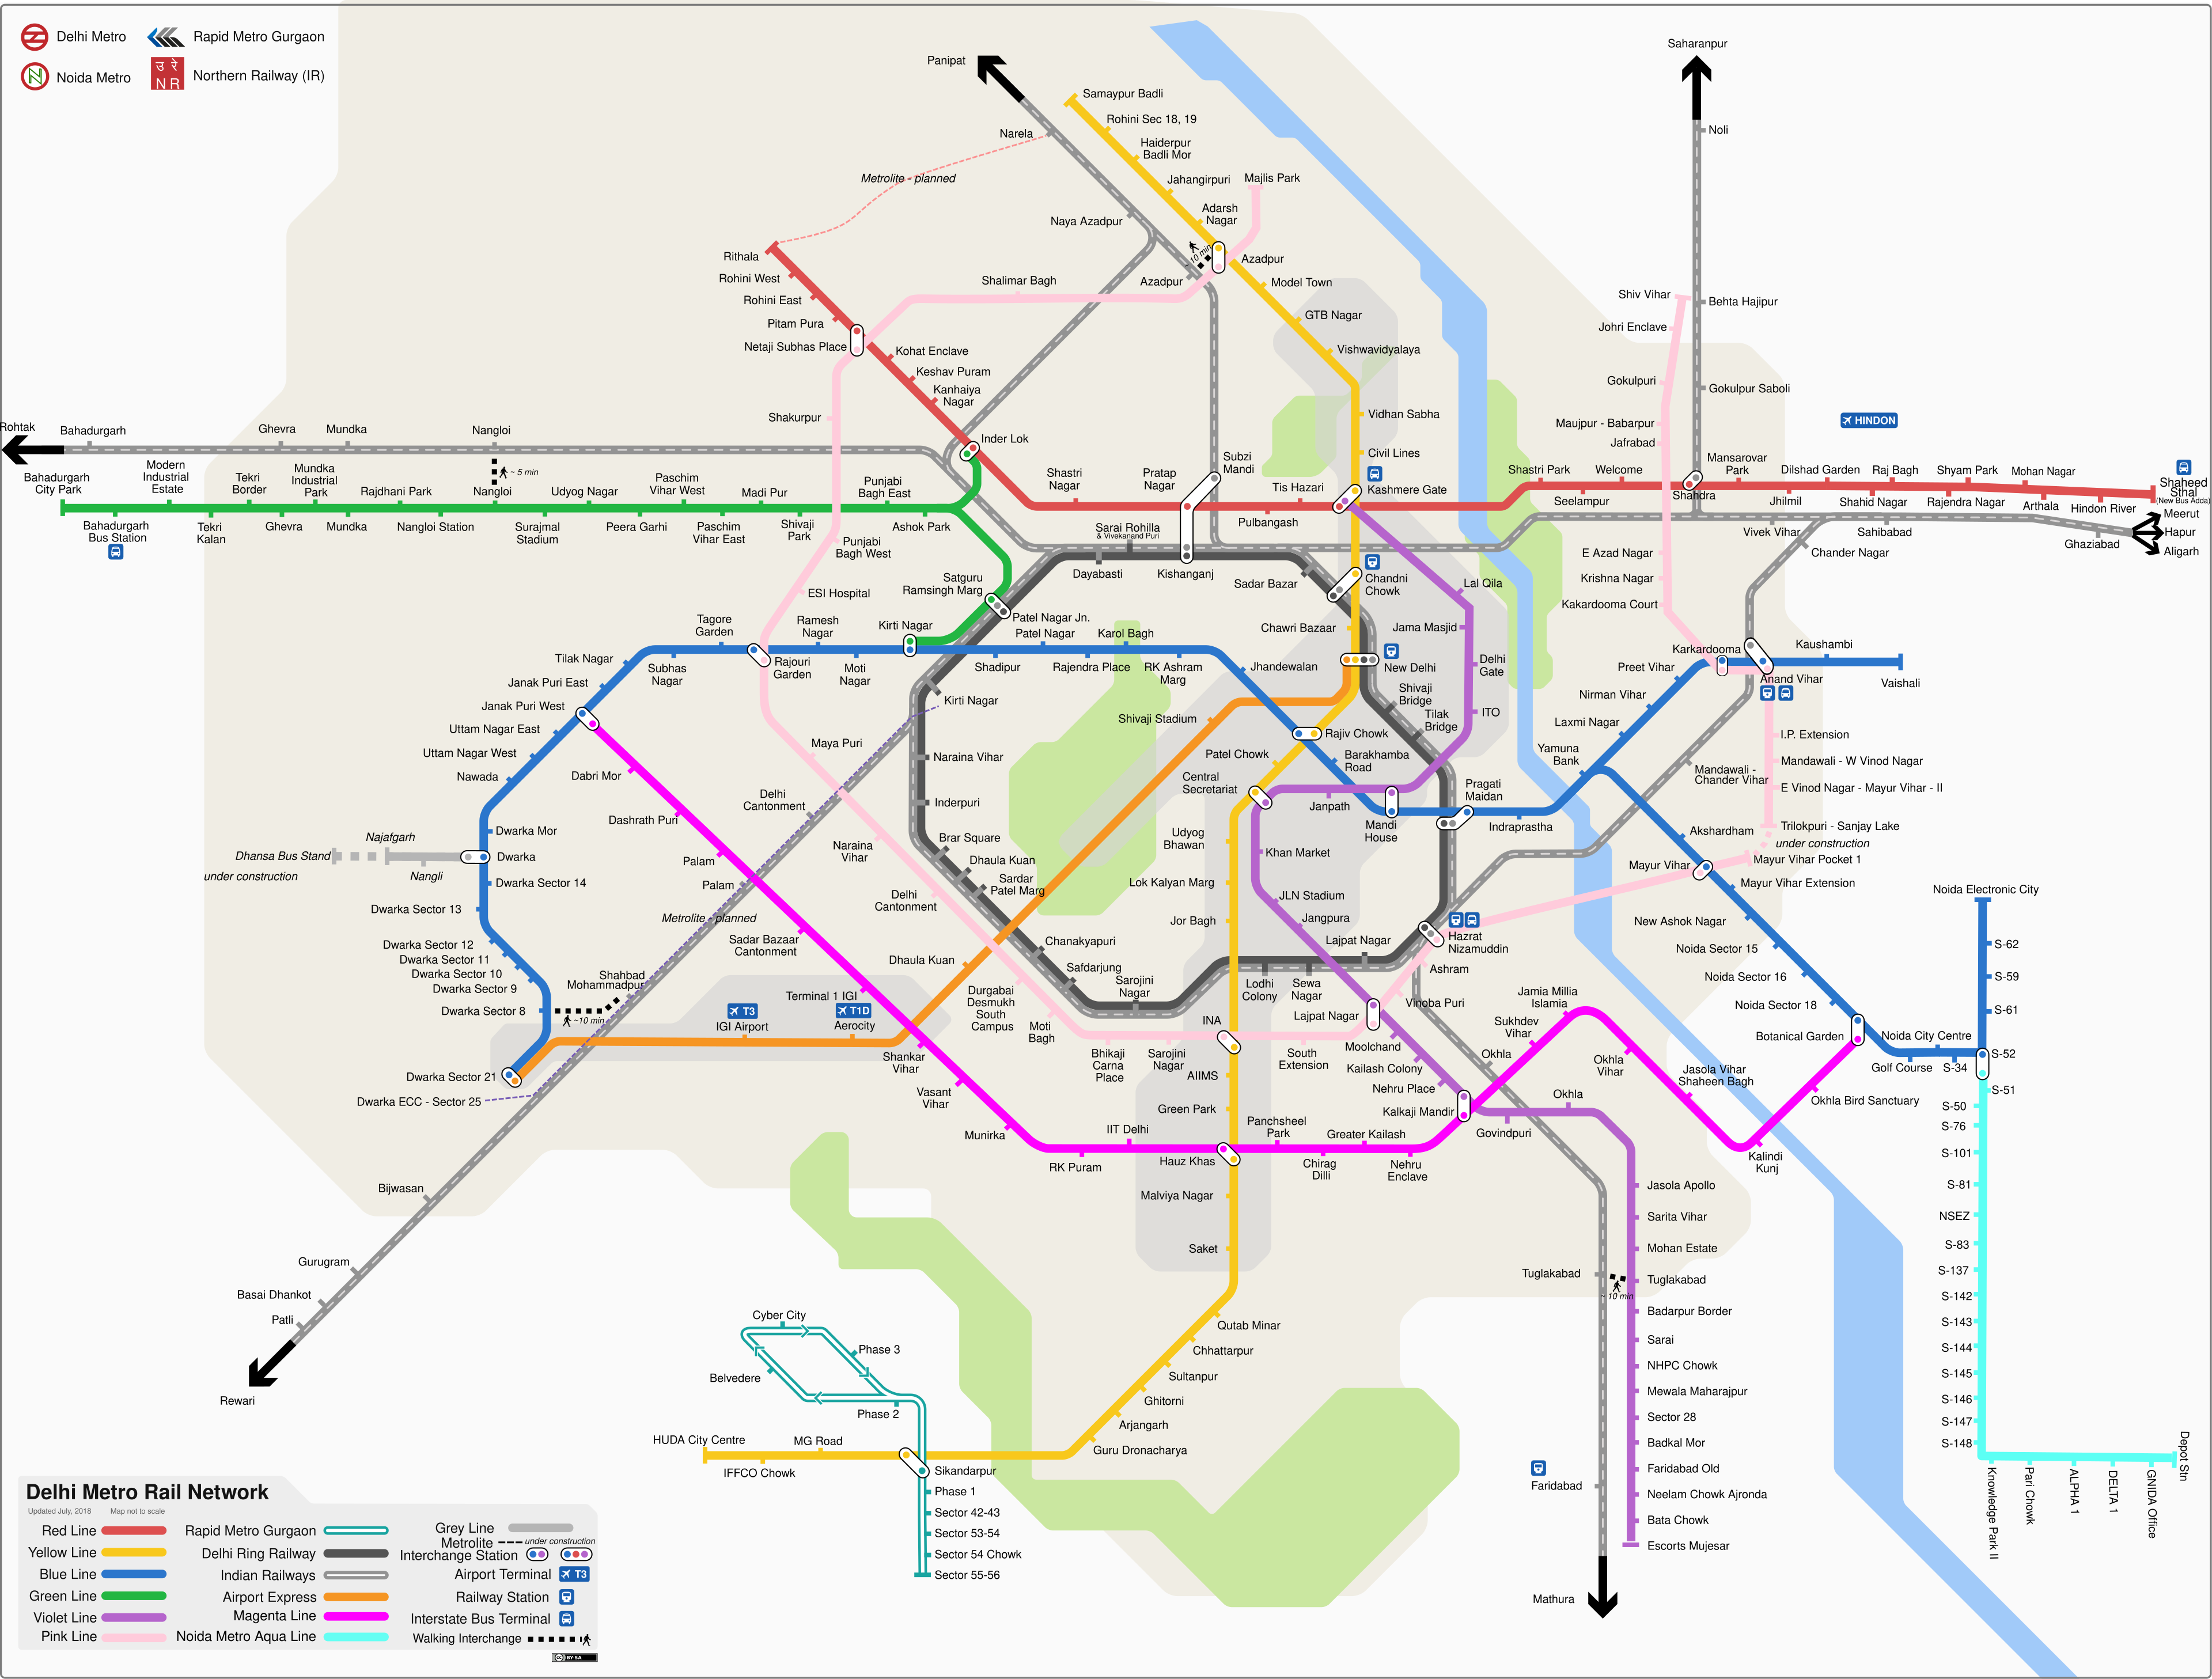
\includegraphics[width=0.6\textwidth]{delhi-metro.png}
  \end{center}
  
  \textit{Question:} How would we figure out a route between two locations? Can we draw it more legibly?
\end{frame}

\begin{frame}
  \frametitle{Example: Erdős Collaboration Network}
  
  \begin{center}
    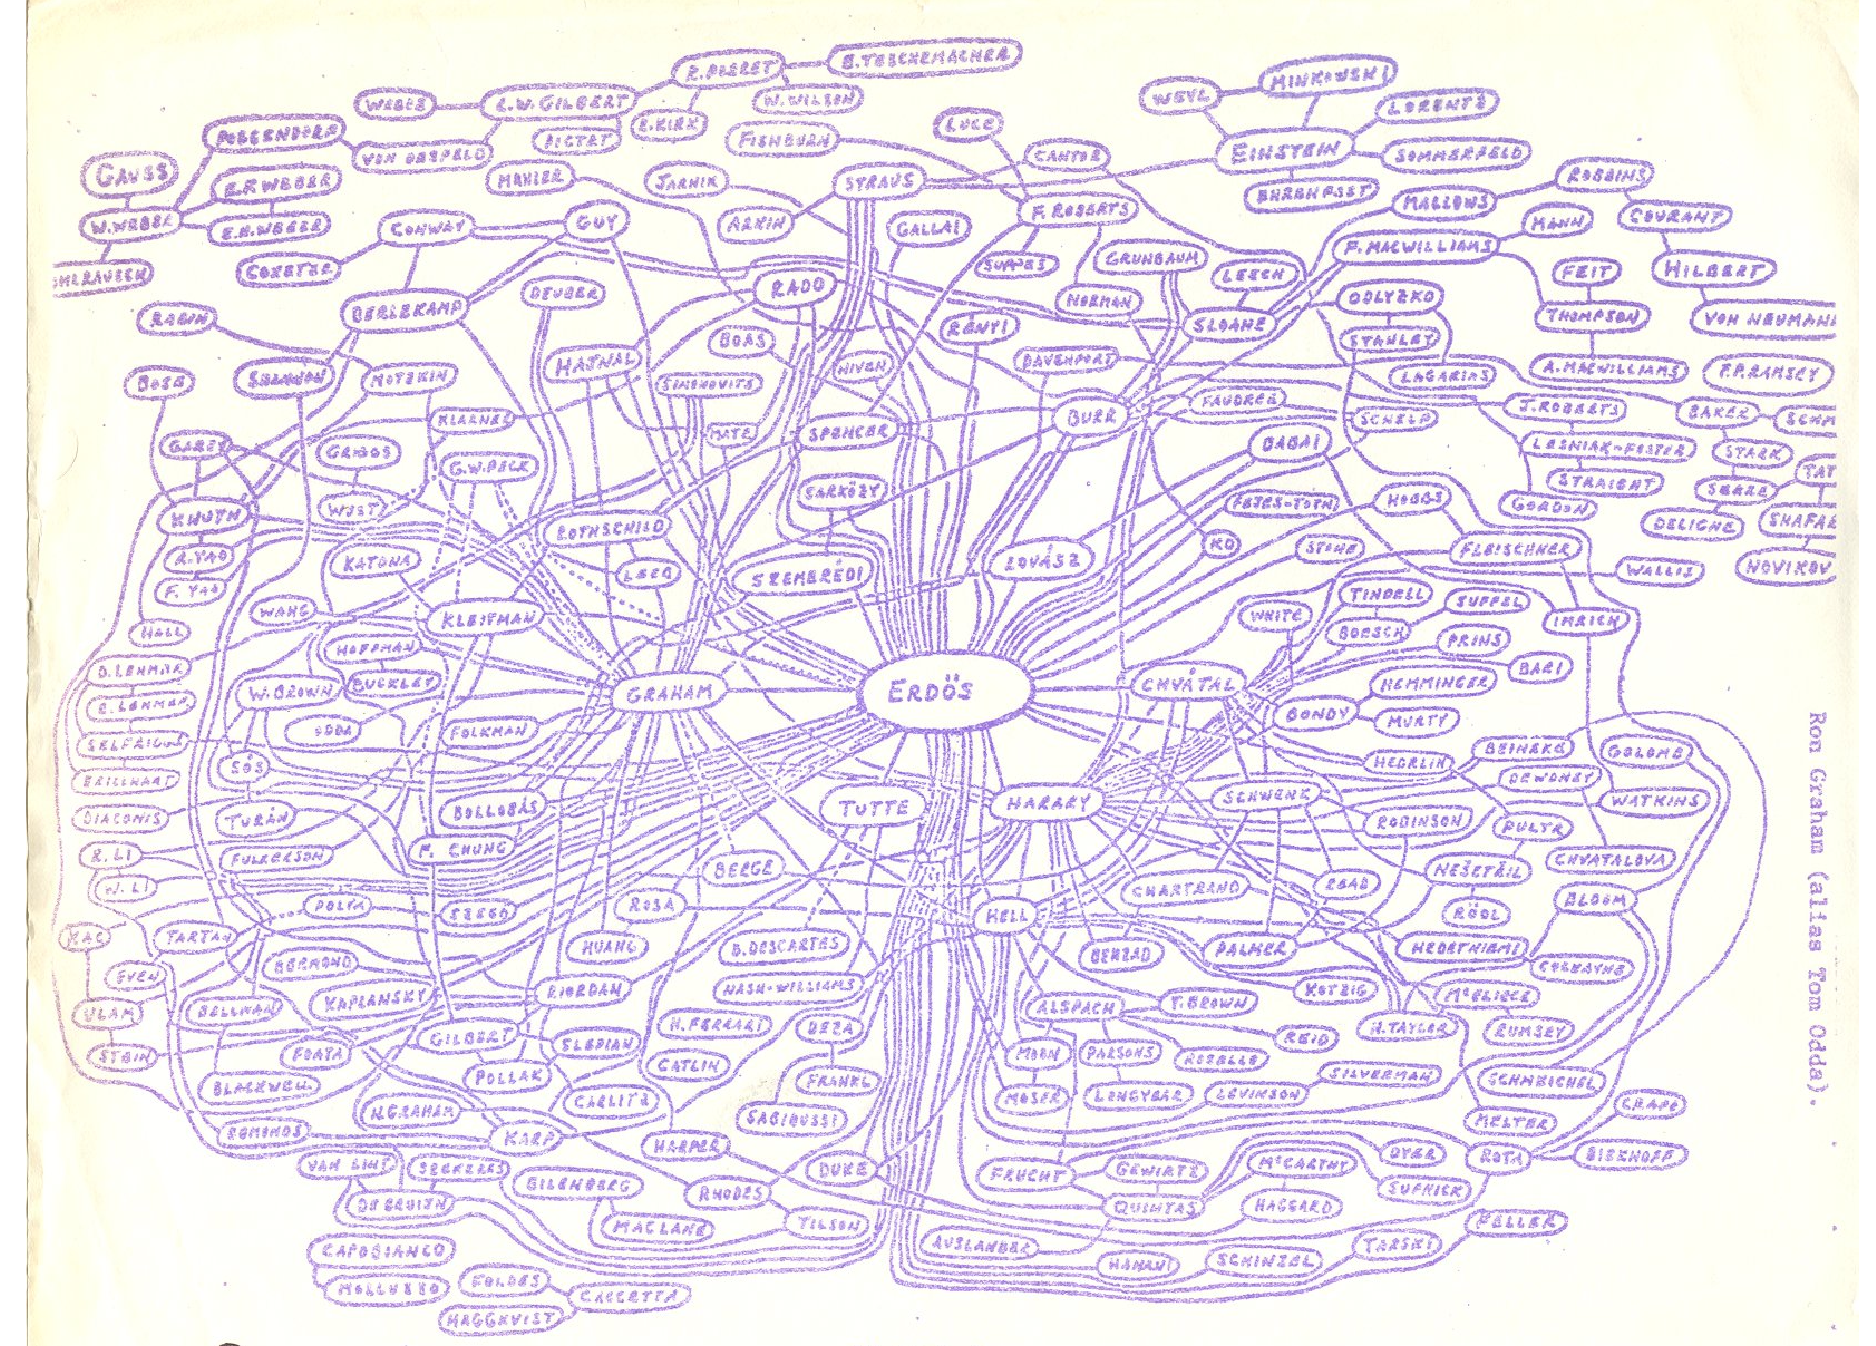
\includegraphics[width=0.6\textwidth]{erdos.png}
  \end{center}
  
  Handdrawn graph of Erdős's collaborations.
  
  \textit{Question:} Given a person, can we find their Erdős number efficiently?
\end{frame}

\begin{frame}
  \frametitle{Example: Chapter Dependencies}
  
  \begin{center}
    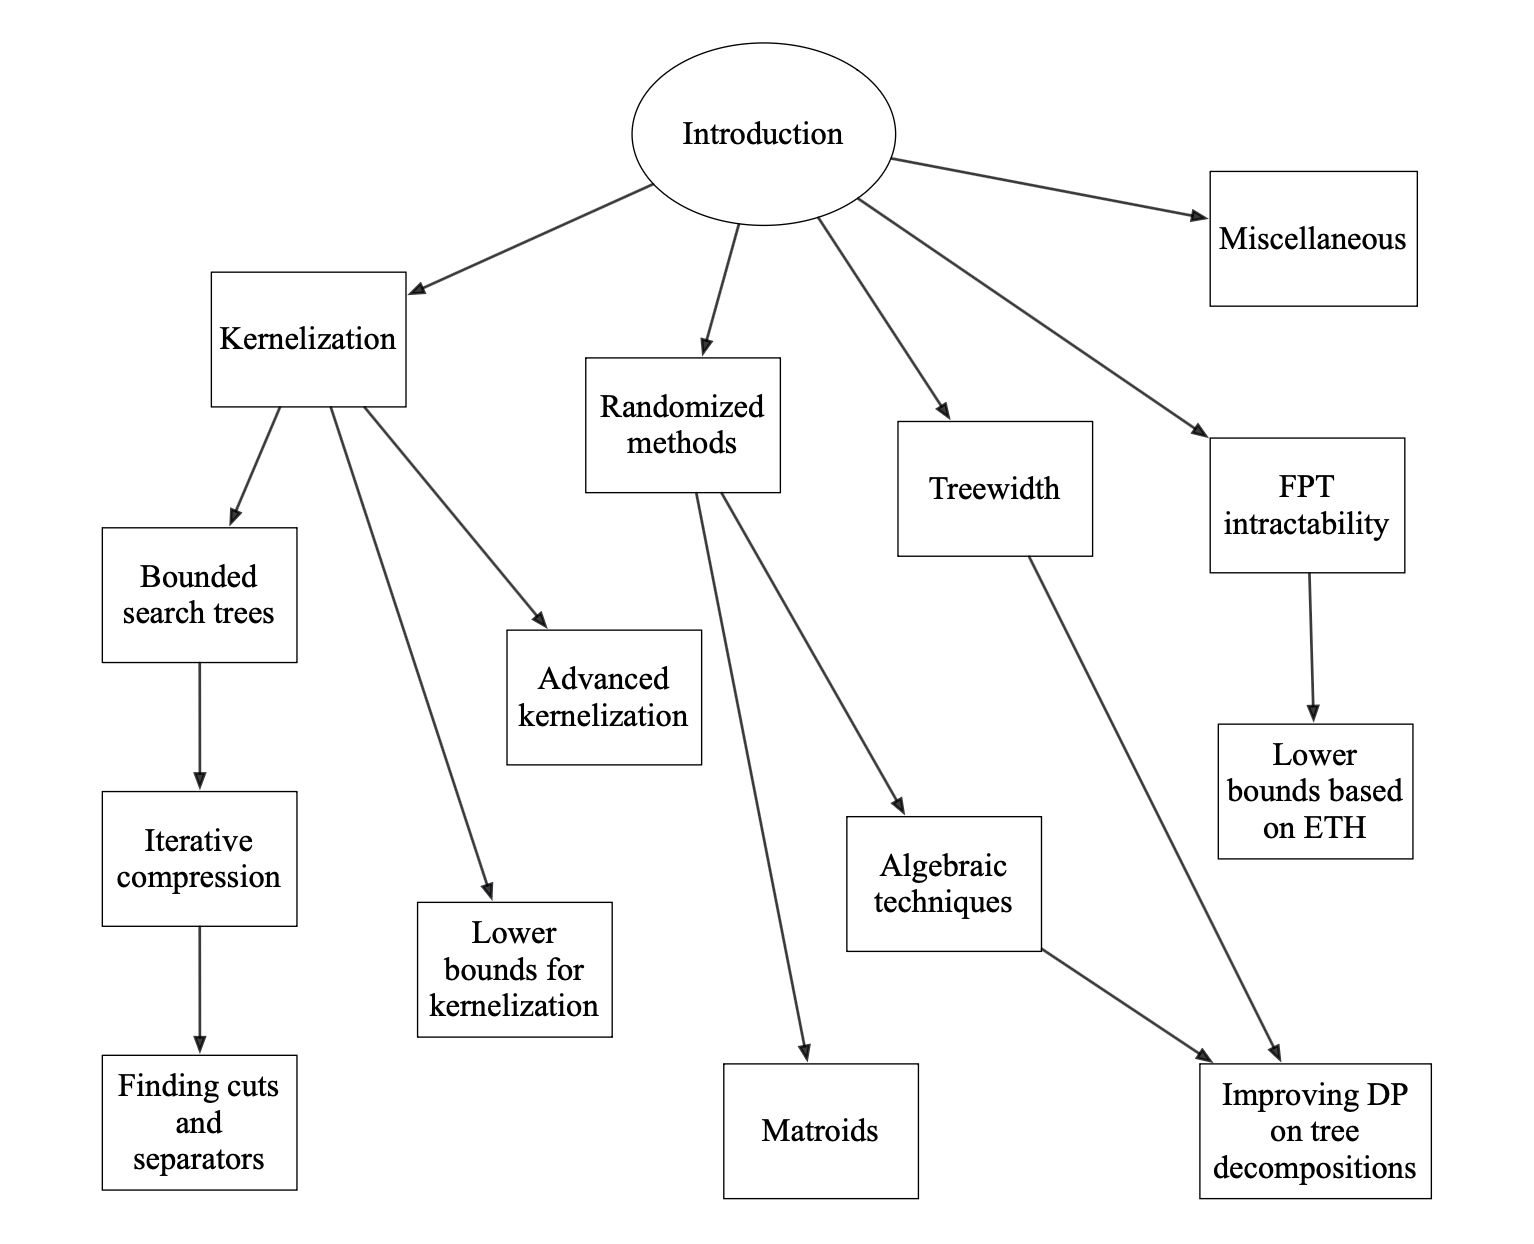
\includegraphics[width=0.5\textwidth]{parametrized-graph.png}
  \end{center}
  
  Chapterwise dependencies from Parametrized Algorithms.
  
  \textit{Questions:} In what order should chapters be read? Which is most important?
\end{frame}

\begin{frame}
  \frametitle{Example: Game Choice Tree}
  
  \begin{center}
    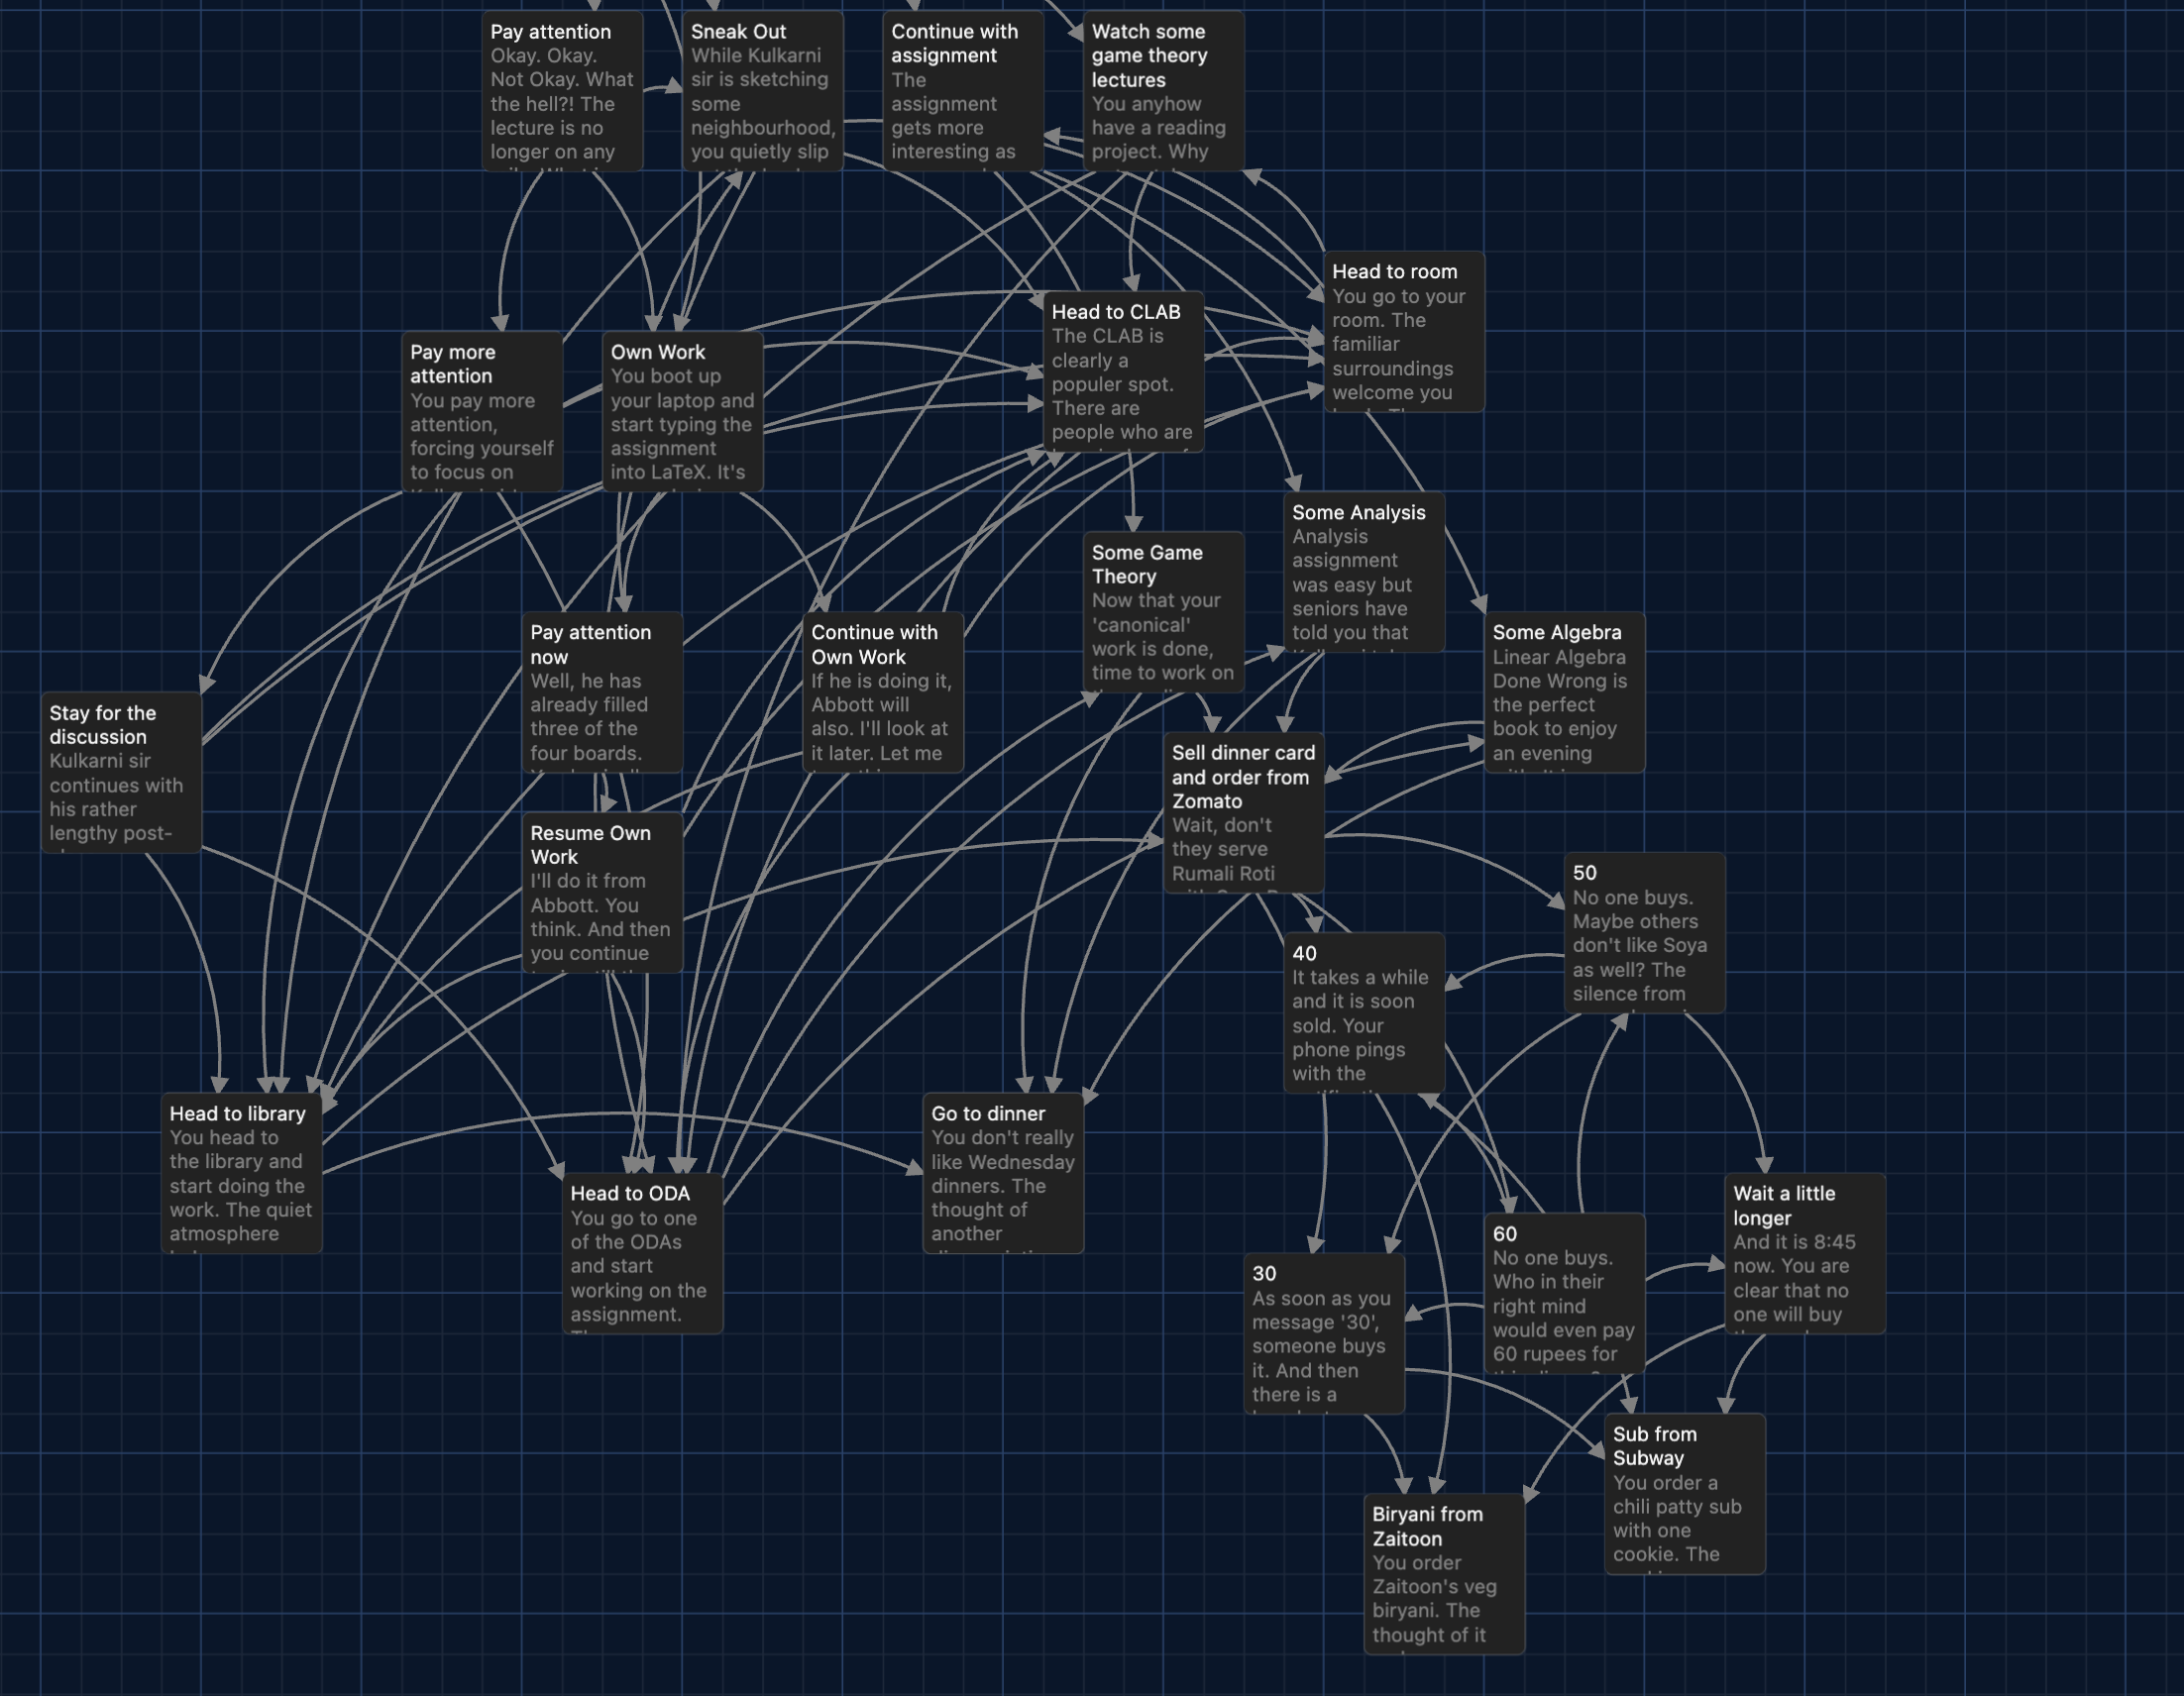
\includegraphics[width=0.6\textwidth]{choice-tree.png}
  \end{center}
  
  Part of a choice tree for a game.
  
  \textit{Questions:} Is there a loop? Which scenes are visited most?
\end{frame}

\begin{frame}
  \frametitle{Example: Indian Rail Network}
  
  \begin{center}
    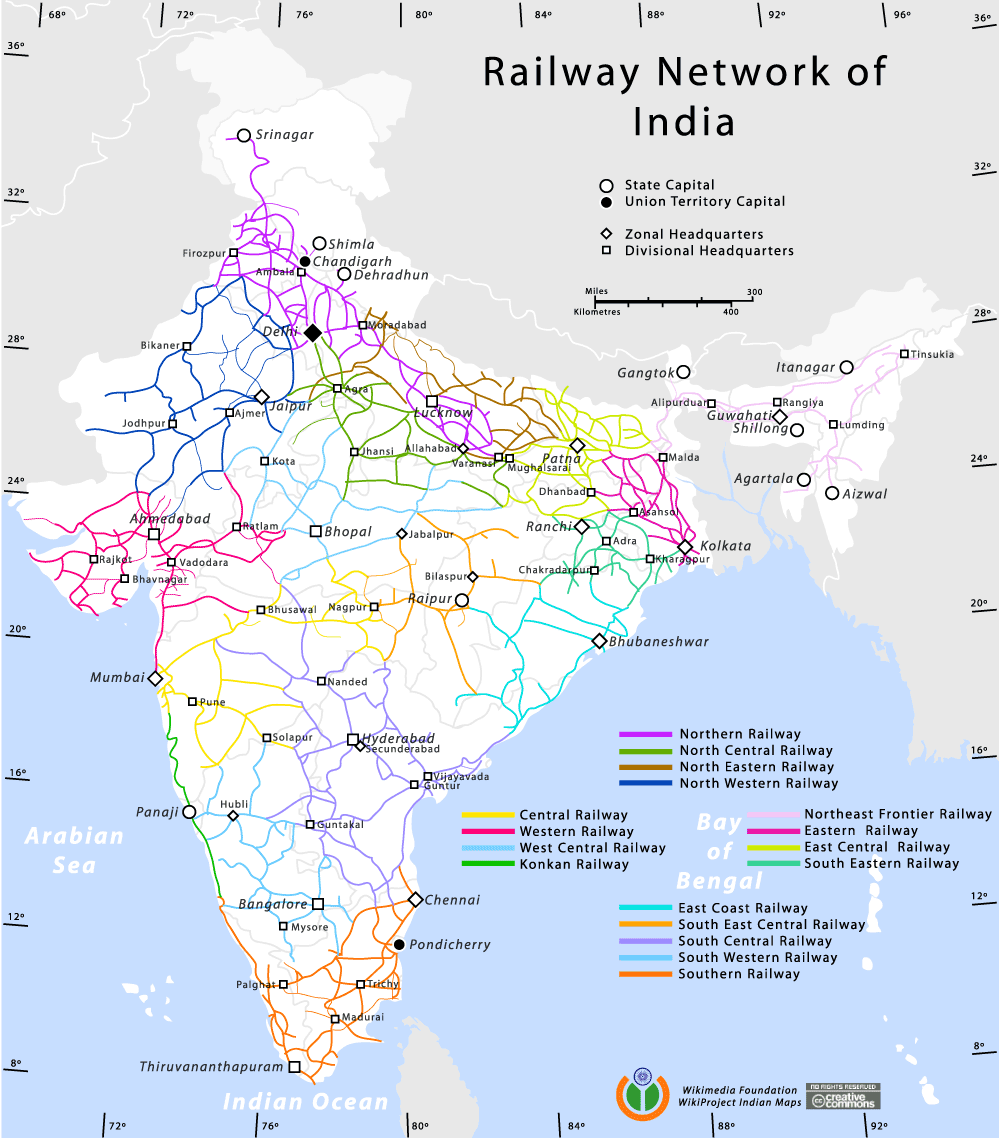
\includegraphics[width=0.4\textwidth]{indian-rail.png}
  \end{center}
  
  Rail network of India.
  
  \textit{Questions:} What is the cheapest/fastest route? Which rails should we shut down to cut costs while maintaining connectivity?
\end{frame}

\begin{frame}
  \frametitle{Core Insight}
  
  There are many graphs and many questions about them:
  \begin{itemize}
    \item Shortest paths
    \item Network connectivity
    \item Centrality and influence
    \item Cycles and trees
    \item Optimal subgraphs
  \end{itemize}
  
  \vspace{0.3cm}
  
  This is what we'll explore in coming classes and tutorials.
\end{frame}

\begin{frame}
  \frametitle{Subgraph}
  
  \begin{definition}
    We say $H = (V', E')$ is a subgraph of $G = (V, E)$ if $V' \subseteq V$ and $E' \subseteq E$.
  \end{definition}
  
  \vspace{0.3cm}
  
  Informally: $H$ is obtained by removing vertices and edges from $G$.
\end{frame}

\begin{frame}
  \frametitle{Adding/Removing Vertices \& Edges}
  
  \begin{definition}
    For an edge $xy$ or vertex $x$:
    \begin{itemize}
      \item $G - xy$ is $G$ with edge $xy$ removed
      \item $G - x$ is $G$ with vertex $x$ and all its incident edges removed
      \item $G + xy$ is $G$ with edge $xy$ added
      \item $G + x$ is $G$ with vertex $x$ added
    \end{itemize}
  \end{definition}
\end{frame}

\begin{frame}
  \frametitle{Neighborhood and Degree}
  
  \begin{definition}
    If $xy \in E$, then $x$ and $y$ are \textbf{adjacent} or \textbf{neighbors}.
    
    The \textbf{neighborhood} of $x$ is: $N(x) = \{y \in V \mid xy \in E\}$
  \end{definition}
  
  \begin{definition}
    The \textbf{degree} of a vertex $x$ is: $\deg(x) = |N(x)|$
    
    This equals the number of edges incident to $x$.
  \end{definition}
\end{frame}

\begin{frame}
  \frametitle{Handshake Lemma}
  
  \begin{lemma}
    For all graphs $G = (V, E)$:
    $$\sum_{v \in V} \deg(v) = 2|E|$$
  \end{lemma}
  
  \begin{proof}
    Every edge contributes to the degrees of exactly 2 vertices. Thus, adding the degrees counts each edge exactly twice.
  \end{proof}
\end{frame}

\begin{frame}
  \frametitle{Your Friends Have More Friends}
  
  \begin{theorem}
    For a graph $G = (V, E)$ with no isolated vertices:
    $$\sum_{v \in V} \deg(v) \leq \sum_{v \in V} \frac{\sum_{n \in N(v)} \deg(n)}{\deg(v)}$$
    
    The average degree of neighbors exceeds the average degree of vertices.
  \end{theorem}
\end{frame}

\begin{frame}
  \frametitle{Proof: Your Friends Have More Friends}
  
  \begin{proof}
    By the Handshake Lemma, LHS $= 2|E|$.
    
    For the RHS:
    \begin{align*}
      \sum_{v \in V} \frac{\sum_{n \in N(v)} \deg(n)}{\deg(v)} &= \sum_{v \in V} \frac{\sum_{uv \in E} \deg(u)}{\deg(v)} \\
      &= \sum_{uv \in E} \left(\frac{\deg(u)}{\deg(v)} + \frac{\deg(v)}{\deg(u)}\right) \\
      &\geq 2|E|
    \end{align*}
    
    The last inequality uses: $\frac{a}{b} + \frac{b}{a} \geq 2$ for all positive $a, b$.
  \end{proof}
\end{frame}

\begin{frame}
  \frametitle{Implications (1): The Comparison Trap}
  
  \textbf{Comparison is truly the thief of joy.}
  
  If you look at:
  \begin{itemize}
    \item The number of friends of your friends
    \item Citations of people you cite
    \item Followers of people you follow
    \item Partners of your partner
  \end{itemize}
  
  You will likely feel sad. The graph gives you good reason to believe everyone else is doing better, but this tells you nothing about how well you're actually doing.
  
  (In many cases, the graph is weighted, and you might not be accounting for the weights!)
\end{frame}

\begin{frame}
  \frametitle{Implications (2): Finding High-Centrality Vertices}
  
  To find a high-centrality individual:
  
  \textbf{Method:} Randomly choose a vertex and randomly choose one of its neighbors.
  
  \vspace{0.3cm}
  
  \textbf{Why this works:}
  \begin{itemize}
    \item The high-degree vertices will be neighbors of many vertices
    \item So they're more likely to be selected
  \end{itemize}
  
  \vspace{0.3cm}
  
  Even better: Choose a vertex and pick its neighbor with highest degree.
  
  \textit{Applications:} Preventing rumors, controlling pandemics.
\end{frame}

\begin{frame}
  \frametitle{Example: Finding Influential People}
  
  \textbf{Instagram Example:}
  
  We can find the most followed person by asking a random person who the most famous person they follow is.
  
  \begin{itemize}
    \item Probability of success: $\approx \frac{678 \text{ million}}{3 \text{ billion}} \approx 0.226$
    \item Much better than random guessing!
  \end{itemize}
  
  \vspace{0.3cm}
  
  \textbf{Time Complexity:}
  \begin{itemize}
    \item Computing all degrees: $O(|V|)$
    \item Random approach: $\mathbb{E}[O(\deg(v))] = O\left(\frac{2|E|}{|V|}\right)$
  \end{itemize}
\end{frame}

\end{document}